\chapter{Permutation, Sorting, and Multiway Merge Sort in External Memory}
\label{cha:lecture-three}

\begin{center}
  \textbf{Lecture 3}\\
  \emph{Permutation vs. Sorting, Multiway Merge Sort, Snow Plow, and Disk Striping}\\[0.5em]
  Date: September 18, 2026
\end{center}

In this chapter, we examine the fundamental relationship between the permutation problem and the sorting problem in the two-level memory hierarchy, contrasting the limitations of the RAM model with block-based storage systems. We analyze the external Binary Merge Sort, highlighting its memory underutilization bottleneck, and develop in detail the \textit{Multiway Merge Sort} ($k$-Way Merge Sort) that achieves the asymptotic lower bound of Aggarwal and Vitter. Finally, we explore two core Algorithm Engineering techniques for secondary storage: optimizing initial runs via the \textit{Snow Plow} algorithm (\textit{Replacement Selection}) and scaling parallel throughput across multiple disks via \textit{Disk Striping}.


\section{The Permutation vs. Sorting Problem}
\label{sec:permutation-vs-sorting}

\subsection{Problem Formulation}
\label{subsec:problem-formulation}

We are given two vectors of size $n$:
\begin{itemize}
  \item A data array $S[1 \dots n]$.
  \item A permutation vector $\pi[1 \dots n]$, containing a bijective permutation of the indices $\{1, 2, \dots, n\}$.
\end{itemize}

The objective is to rearrange the elements of $S$ into a new array $S'$ such that each original element $S[i]$ is placed into the destination position specified by $\pi[i]$:
\begin{equation}
  S'[\pi[i]] = S[i], \qquad \forall i \in \{1, \dots, n\}.
\end{equation}

\begin{example}[Index Permutation]
\label{ex:permutation-def}
Consider an array of $4$ elements and its corresponding permutation vector:
\begin{align*}
  \text{Indices:} \quad & 1 \quad 2 \quad 3 \quad 4 \\
  S = \quad & [\, A, \quad B, \quad C, \quad D \,] \\
  \pi = \quad & [\, 3, \quad 1, \quad 2, \quad 4 \,]
\end{align*}
Applying the definition element by element:
\begin{align*}
  S'[\pi[1]] &= S'[3] = A, \\
  S'[\pi[2]] &= S'[1] = B, \\
  S'[\pi[3]] &= S'[2] = C, \\
  S'[\pi[4]] &= S'[4] = D.
\end{align*}
The resulting permuted array is therefore:
\[
  S' = [\, B, \quad C, \quad A, \quad D \,].
\]
\end{example}

In \autoref{fig:permutation-example}, the mapping from the source array to the destination array is illustrated visually.

\begin{figure}[H]
  \centering
  \begin{tikzpicture}[
    box/.style={draw, thick, minimum width=1.45cm, minimum height=0.72cm, align=center, font=\small},
    hdr/.style={font=\small\bfseries, anchor=east},
    arr/.style={-{Stealth[scale=1.1]}, thick}
  ]
    % Row headers on left
    \node[hdr] at (-0.6, 2.8) {Index $i$:};
    \node[hdr] at (-0.6, 2.0) {Element $S[i]$:};
    \node[hdr] at (-0.6, 1.2) {Target $\pi[i]$:};

    % Original array S and permutation vector columns
    \foreach \x/\i/\val/\dest in {0.5/1/A/3, 2.7/2/B/1, 4.9/3/C/2, 7.1/4/D/4} {
      \node[box, fill=gray!8] (idx\i) at (\x, 2.8) {$i = \i$};
      \node[box, fill=blue!12] (S\i) at (\x, 2.0) {\textbf{\val}};
      \node[box, fill=orange!15] (P\i) at (\x, 1.2) {$\pi[\i] = \dest$};
    }

    % Row headers for permuted array S'
    \node[hdr] at (-0.6, -1.8) {Array $S'$:};
    \node[hdr] at (-0.6, -2.6) {Index $j$:};

    % Permuted array S' cells
    \foreach \x/\j/\val in {0.5/1/B, 2.7/2/C, 4.9/3/A, 7.1/4/D} {
      \node[box, fill=green!15] (Sp\j) at (\x, -1.8) {\textbf{\val}};
      \node[box, fill=gray!8] (tgt\j) at (\x, -2.6) {$j = \j$};
    }

    % Relocation arrows with white-background labels
    \draw[arr, color=blue!75!black] (P1.south) to[out=270,in=90] 
      node[pos=0.45, right=1pt, font=\scriptsize, fill=white, inner sep=1.5pt] {$S[1] \to S'[3]$} (Sp3.north);

    \draw[arr, color=red!75!black] (P2.south) to[out=270,in=90] 
      node[pos=0.45, left=1pt, font=\scriptsize, fill=white, inner sep=1.5pt] {$S[2] \to S'[1]$} (Sp1.north);

    \draw[arr, color=orange!85!black] (P3.south) to[out=270,in=90] 
      node[pos=0.55, right=1pt, font=\scriptsize, fill=white, inner sep=1.5pt] {$S[3] \to S'[2]$} (Sp2.north);

    \draw[arr, color=teal!85!black] (P4.south) to[out=270,in=90] 
      node[pos=0.5, right=1pt, font=\scriptsize, fill=white, inner sep=1.5pt] {$S[4] \to S'[4]$} (Sp4.north);
  \end{tikzpicture}
  \caption{Permutation mapping: each element $S[i]$ is relocated to the destination index specified by $\pi[i]$ in array $S'$.}
  \label{fig:permutation-example}
\end{figure}

\subsection{Naive Implementation on the RAM Model}
\label{subsec:naive-ram}

In the standard RAM model, where any read or write access to arbitrary memory locations costs $\mathcal{O}(1)$ time, the permutation is implemented in a single linear pass:

\begin{algorithm}[H]
  \DontPrintSemicolon
  \KwInput{Array $S[1 \dots n]$, permutation vector $\pi[1 \dots n]$}
  \KwOutput{Permuted array $S$ in place}
  \For{$i \leftarrow 1$ \KwTo $n$}{
    $S'[\pi[i]] \leftarrow S[i]$\;
  }
  $S \leftarrow \mathrm{copy}(S')$\;
  \caption{Direct Permutation on RAM}
\end{algorithm}

The time complexity in the RAM model is strictly linear:
\[
  T_{\mathrm{RAM}}(n) = \Theta(n).
\]
Therefore, in internal memory, permuting is asymptotically faster than sorting by comparisons, which requires $\Omega(n \log n)$ operations.

\subsection{Simulation Principle (RAM to Two-Level Memory)}
\label{subsec:simulation-principle}

\begin{theorem}[Simulation Theorem]
\label{thm:simulation}
Any sequential algorithm formulated for the RAM model with time complexity $T(n)$ incurs at most $\mathcal{O}(T(n))$ block transfers (I/Os) in the two-level memory model with parameters $(M, B)$.
\end{theorem}

\begin{proof}[Proof Sketch]
In the worst case, every single RAM operation accessing memory addresses a memory cell that resides in a block not currently resident in internal cache $M$. Each such access triggers a block transfer from disk, resulting in exactly $1$ I/O operation. Multiplying the total step count $T(n)$ by the upper bound of $1$ I/O per step yields the trivial bound of $\mathcal{O}(T(n))$ I/Os.
\end{proof}

Although the simulation principle guarantees that any RAM algorithm can be ported to external memory, the bound $\mathcal{O}(T(n))$ is often thoroughly sub-optimal because it fails to exploit the block aggregation factor $B$.

\subsection{The Relationship Between Sorting and Permutation}
\label{subsec:relationship-sort-perm}

In the two-level memory hierarchy, the complexity relationship changes fundamentally, as summarized in \autoref{tab:ram-vs-twlevel}:

\begin{table}[H]
  \centering
  \renewcommand{\arraystretch}{1.5}
  \resizebox{0.94\linewidth}{!}{%
  \begin{tabular}{lcc}
    \toprule
    \textbf{Problem} & \textbf{RAM Model} & \textbf{Two-Level Memory (I/O)} \\
    \midrule
    \textbf{Permutation} $\operatorname{Perm}(n)$ & $\Theta(n)$ & $\Theta\big(\min\big\{ n, \, \operatorname{Sort}(n, M, B) \big\}\big)$ \\[0.4em]
    \textbf{Sorting} $\operatorname{Sort}(n)$ & $\Theta(n \log_2 n)$ & $\displaystyle \Theta\left(\frac{n}{B} \log_{M/B} \frac{n}{B}\right)$ \\
    \bottomrule
  \end{tabular}%
  }
  \caption{Asymptotic complexity comparison between RAM and External Memory models.}
  \label{tab:ram-vs-twlevel}
\end{table}

To understand this equivalence in block-based storage, consider the two reductions:

\begin{enumerate}
  \item \textbf{Sorting via Permutation:} Given an array $S$, sorting requires computing the permutation $\pi_S$ that puts keys in order, and then applying $\pi_S$ to $S$.
  \item \textbf{Permuting via Sorting (Pair Reduction Algorithm):}
  Permuting an array $S$ can be converted into an external sorting problem via the following three-step procedure:
  \begin{itemize}
    \item \textbf{Step 1 (Scan and Pair Creation):} Perform parallel linear scans over $S$ and $\pi$ to construct a set of $n$ records containing $\langle S[i], \pi[i] \rangle$. Since this requires only streaming sequential I/O, the cost is:
    \[
      \mathrm{I/O}_{\text{Step 1}} = \mathcal{O}\left(\frac{n}{B}\right).
    \]
    \item \textbf{Step 2 (Sorting by Destination):} Sort the $n$ records using the second component $\pi[i]$ as the sorting key. The cost is identical to external sorting:
    \[
      \mathrm{I/O}_{\text{Step 2}} = \operatorname{Sort}(n, M, B).
    \]
    \item \textbf{Step 3 (Scan and Extraction):} Since the records are now sorted by increasing target index, a simple sequential scan extracts the first coordinate $S[i]$ into the destination array $S'$. The cost is:
    \[
      \mathrm{I/O}_{\text{Step 3}} = \mathcal{O}\left(\frac{n}{B}\right).
    \]
  \end{itemize}
\end{enumerate}

The overall I/O cost of this reduction is:
\begin{equation}
  \mathrm{I/O}_{\text{Sort-based}} = \mathcal{O}\left(\frac{n}{B}\right) + \operatorname{Sort}(n, M, B) + \mathcal{O}\left(\frac{n}{B}\right) = \Theta(\operatorname{Sort}(n, M, B)).
\end{equation}

\begin{example}[Step-by-Step Pair Reduction Trace on Concrete Arrays]
\label{ex:pair-reduction-trace}
To visualize the reduction with concrete values, consider the instance from \autoref{ex:permutation-def}:
\[
  S = [A, B, C, D], \qquad \pi = [3, 1, 2, 4].
\]
The algorithm executes across three sequential states of the record array:
\begin{itemize}
  \item \textbf{Step 1 (Pairing):} Sequentially pair each item with its designated target index:
  \[
    P = \big[ \, \langle A, 3 \rangle, \;\; \langle B, 1 \rangle, \;\; \langle C, 2 \rangle, \;\; \langle D, 4 \rangle \, \big].
  \]
  \item \textbf{Step 2 (External Sorting on $\pi[i]$):} Sort the record array using the second coordinate (target destination) as the sorting key:
  \[
    P_{\text{sorted}} = \big[ \, \langle B, \mathbf{1} \rangle, \;\; \langle C, \mathbf{2} \rangle, \;\; \langle A, \mathbf{3} \rangle, \;\; \langle D, \mathbf{4} \rangle \, \big].
  \]
  \item \textbf{Step 3 (Sequential Extraction):} Stream through the sorted records and project their first coordinates to form the destination array:
  \[
    S' = [B, C, A, D],
  \]
  which correctly fulfills the required permutation since $S'[1]=B$, $S'[2]=C$, $S'[3]=A$, $S'[4]=D$.
\end{itemize}
\end{example}

The pair reduction pipeline is illustrated in \autoref{fig:pair-reduction}.

\begin{figure}[H]
  \centering
  \begin{tikzpicture}[
    node distance=0.55cm and 0cm,
    data/.style={draw=blue!60!black, fill=blue!6, rounded corners=4pt, font=\small, align=center, inner sep=5pt, minimum width=6.2cm},
    stepnode/.style={draw=orange!80!black, fill=orange!10, rounded corners=4pt, font=\small\bfseries, align=center, inner sep=5pt, minimum width=7.2cm},
    outdata/.style={draw=teal!70!black, fill=teal!10, rounded corners=4pt, font=\small\bfseries, align=center, inner sep=5pt, minimum width=6.2cm},
    arr/.style={-{Stealth[scale=1.1]}, thick, draw=gray!70!black}
  ]
    \node[data] (in) {Input Data\\Array $S[1\dots n]$ \quad and \quad Vector $\pi[1\dots n]$};
    \node[stepnode, below=of in] (s1) {Step 1: Sequential Pairing\\{\normalfont\footnotesize Cost: $\mathcal{O}(n/B)$ I/Os (streaming linear scan)}};
    \node[data, below=of s1] (pairs) {Collection of Unordered Pairs\\$\big\{ \langle S[i], \pi[i] \rangle \;\mid\; i = 1, \dots, n \big\}$};
    \node[stepnode, below=of pairs] (s2) {Step 2: External Sort on $\pi[i]$\\{\normalfont\footnotesize Cost: $\operatorname{Sort}(n, M, B)$ I/Os (External Merge Sort)}};
    \node[data, below=of s2] (spairs) {Pairs Sorted by Destination Index\\$\big\{ \langle S[\pi^{-1}[j]], j \rangle \;\mid\; j = 1, \dots, n \big\}$};
    \node[stepnode, below=of spairs] (s3) {Step 3: Sequential Extraction\\{\normalfont\footnotesize Cost: $\mathcal{O}(n/B)$ I/Os (sequential write)}};
    \node[outdata, below=of s3] (out) {Final Permuted Array\\$S'[1\dots n]$ \quad with \quad $S'[\pi[i]] = S[i]$};

    \draw[arr] (in) -- (s1);
    \draw[arr] (s1) -- (pairs);
    \draw[arr] (pairs) -- (s2);
    \draw[arr] (s2) -- (spairs);
    \draw[arr] (spairs) -- (s3);
    \draw[arr] (s3) -- (out);
  \end{tikzpicture}
  \caption{Operational workflow of the pair-reduction permutation algorithm.}
  \label{fig:pair-reduction}
\end{figure}

\section[Permutation Complexity in External Memory]{Permutation Complexity\\in External Memory}
\label{sec:permutation-complexity}

The fundamental lower bound for permutation in the two-level memory model was established by Aggarwal and Vitter~\cite{aggarwal1988}:
\begin{equation}
  \operatorname{Perm}(n, M, B) = \Theta\left(\min\left\{ n, \, \frac{n}{B} \log_{M/B}\left(\frac{n}{B}\right) \right\}\right).
\end{equation}
Letting $L = \log_{M/B}(n/B)$ denote the number of merge passes required by multiway merge sort:
\begin{equation}
  \operatorname{Sort}(n, M, B) = \Theta\left(\frac{n}{B} \cdot L\right).
\end{equation}

\subsection{Corner Case Analysis}
\label{subsec:corner-cases}

Comparing the direct naive algorithm with the sorting-based reduction yields two distinct regimes determined by the relationship between block size $B$ and pass count $L$:
\begin{itemize}
  \item \textbf{Case 1 ($n \ge \frac{n}{B} \cdot L \iff B \ge L$):}  
  The block size $B$ is greater than or equal to the depth of the merge tree. In this setting, sorting the pairs requires fewer I/Os than random single-element access:
  \[
    \operatorname{Perm}(n, M, B) = \Theta(\operatorname{Sort}(n, M, B)).
  \]
  \item \textbf{Case 2 ($n < \frac{n}{B} \cdot L \iff B < L$):}  
  If the block size were pathologically small compared to the overall dataset ($B < L$), direct element-by-element random writing (at most $n$ I/Os) would be asymptotically cheaper than sorting:
  \[
    \operatorname{Perm}(n, M, B) = \Theta(n).
  \]
\end{itemize}

\subsection{Numerical Verification on Realistic Architectural Parameters}
\label{subsec:numerical-check}

To establish which regime governs real-world computing systems, consider extreme yet realistic parameters:
\begin{itemize}
  \item Fast internal memory: $M = 16\text{ GB} = 2^4 \cdot 2^{30} = 2^{34}$ elements.
  \item Disk block size: $B = 32\text{ KB} = 2^5 \cdot 2^{10} = 2^{15}$ elements.
  \item Input dataset size: $n = 2^{60}$ elements (Exabyte scale).
\end{itemize}

We calculate the merge depth $L$:
\[
  L = \log_{M/B}\left(\frac{n}{M}\right) = \frac{\log_2(n / M)}{\log_2(M / B)}.
\]
Substituting the exponential values:
\begin{align*}
  \frac{n}{M} &= \frac{2^{60}}{2^{34}} = 2^{26} \implies \log_2\left(\frac{n}{M}\right) = 26, \\
  \frac{M}{B} &= \frac{2^{34}}{2^{15}} = 2^{19} \implies \log_2\left(\frac{M}{B}\right) = 19.
\end{align*}
Hence:
\[
  L = \frac{26}{19} \approx 1.36 < 2.
\]
Because $B = 2^{15} = 32\,768$ and $L \le 2$, the condition $B \ge L$ holds by more than four orders of magnitude ($32\,768 \gg 2$). Consequently, in all practical systems, permutation is strictly bound by sorting complexity:
\[
  \operatorname{Perm}(n) = \Theta(\operatorname{Sort}(n)).
\]

\section{External Memory Binary Merge Sort}
\label{sec:binary-merge-sort}

The classical recursive Merge Sort algorithm extends naturally to external memory by recursively dividing arrays, ordering runs, and merging sorted sub-arrays:

\begin{algorithm}[H]
  \DontPrintSemicolon
  \KwInput{Array $S$, boundaries $i, j$}
  \KwOutput{Sorted sub-array $S[i \dots j]$}
  \If{$i < j$}{
    $m \leftarrow \lfloor (i + j) / 2 \rfloor$\;
    $\mathrm{MS}(S, i, m)$\;
    $\mathrm{MS}(S, m + 1, j)$\;
    $\mathrm{MERGE}(S, i, m, j)$\;
  }
  \caption{Binary Merge Sort}
\end{algorithm}

\subsection{Buffer Architecture in the Merge Procedure}
\label{subsec:merge-procedure}

Given two consecutive sorted runs of length $l$, the merge procedure produces a single consolidated run of length $2l$ into an auxiliary array $S'$.

\begin{itemize}
  \item \textbf{In the RAM Model:} The operation performs at most $2l$ comparisons and $2l$ memory writes, costing $\Theta(l)$ CPU steps.
  \item \textbf{In the Two-Level Model:} To minimize block transfers, internal memory $M$ is partitioned into $3$ dedicated buffers, each having size exactly equal to one block $B$:
  \begin{enumerate}
    \item \textbf{Input Buffer 1:} holds one block (size $B$) of the first sorted run.
    \item \textbf{Input Buffer 2:} holds one block (size $B$) of the second sorted run.
    \item \textbf{Output Buffer:} accumulates merged elements in sorted order until full ($B$ elements).
  \end{enumerate}
\end{itemize}

\autoref{fig:merge-buffers} illustrates the internal memory allocation and streaming I/O pattern during the binary merge.

\begin{figure}[H]
  \centering
  \begin{tikzpicture}[
    buf/.style={draw, thick, fill=blue!10, minimum width=3.0cm, minimum height=1.1cm, align=center, font=\small},
    disk/.style={draw, thick, fill=gray!15, minimum width=3.0cm, minimum height=0.9cm, align=center, font=\small},
    arr/.style={-{Stealth[scale=1.1]}, thick}
  ]
    % Internal Memory Container
    \draw[dashed, thick, color=blue!70!black, fill=blue!2] (-0.5, 1.8) rectangle (10.5, 3.8);
    \node[anchor=west, font=\bfseries\small, color=blue!70!black] at (-0.3, 3.5) {Internal Memory $M$ (Space used: $3B$)};

    % Internal buffers
    \node[buf] (b1) at (1.5, 2.6) {Input Buffer 1\\(size $B$)};
    \node[buf] (b2) at (5.0, 2.6) {Input Buffer 2\\(size $B$)};
    \node[buf, fill=green!15] (bout) at (8.5, 2.6) {Output Buffer\\(size $B$)};

    % External runs on disk
    \node[disk] (d1) at (1.5, 0.2) {Run 1 on Disk\\(length $l$)};
    \node[disk] (d2) at (5.0, 0.2) {Run 2 on Disk\\(length $l$)};
    \node[disk, fill=green!8] (dout) at (8.5, 0.2) {Merged Run on Disk\\(length $2l$)};

    % Connections
    \draw[arr, color=blue!80!black] (d1) -- node[right, font=\scriptsize]{Read $B$} (b1);
    \draw[arr, color=blue!80!black] (d2) -- node[right, font=\scriptsize]{Read $B$} (b2);
    \draw[arr, color=green!60!black] (bout) -- node[right, font=\scriptsize]{Flush $B$} (dout);

    % Internal logic
    \draw[thick, dotted, color=gray!80!black] (b1.east) -- (b2.west);
    \draw[thick, dotted, color=gray!80!black] (b2.east) -- (bout.west);
  \end{tikzpicture}
  \caption{Internal memory buffer organization during binary external merge.}
  \label{fig:merge-buffers}
\end{figure}

The execution protocol proceeds as follows:
\begin{enumerate}
  \item The leading elements of the two input buffers are compared in CPU; the smaller key is appended to the output buffer.
  \item Whenever an input buffer is exhausted, a disk read loads the next block of that run ($\frac{l}{B}$ I/Os per input run).
  \item As soon as the output buffer fills up with $B$ items, it is flushed to disk in a single write operation ($\frac{2l}{B}$ write I/Os overall).
\end{enumerate}

The total I/O cost of merging two runs of length $l$ is:
\begin{equation}
  \mathrm{I/O}_{\text{Merge}}(l) = \frac{l}{B} + \frac{l}{B} + \frac{2l}{B} = \frac{4l}{B} = \Theta\left(\frac{l}{B}\right).
\end{equation}

\subsection{Recursion Tree Complexity}
\label{subsec:recursion-tree}

Recursion terminates once sub-array sizes fit entirely within internal memory $M$. At this base level, each chunk of size $M$ is read into memory, sorted using an in-memory algorithm (e.g., QuickSort or HeapSort) with zero additional I/O, and written back to disk using $\mathcal{O}(M/B)$ I/Os.

This yields:
\[
  N_{\mathrm{run}} = \frac{n}{M} \text{ initial sorted runs of size } M.
\]
The binary merge tree has height:
\begin{equation}
  h = \log_2\left(\frac{n}{M}\right) \text{ levels}.
\end{equation}

\autoref{fig:binary-merge-tree} depicts the recursion structure of binary external merge sort.

\begin{figure}[H]
  \centering
  \resizebox{0.95\linewidth}{!}{%
  \begin{tikzpicture}[
    level 1/.style={sibling distance=3.6cm, level distance=1.2cm},
    level 2/.style={sibling distance=1.8cm, level distance=1.2cm},
    node/.style={draw=blue!70!black, rounded corners=3pt, fill=blue!8, font=\small, minimum width=1.5cm, minimum height=0.6cm, align=center},
    leaf/.style={draw=yellow!70!black, rounded corners=3pt, fill=yellow!25, font=\small, minimum width=1.4cm, minimum height=0.6cm, align=center},
    cost/.style={font=\small, text=blue!80!black, anchor=west},
    lbl/.style={font=\small\bfseries, text=gray!75!black, anchor=east}
  ]
    % Tree (centered at x = -1.2)
    \node[node] at (-1.2, 0) (root) {Output: $n$}
      child { node[node] (n1) {Run $n/2$}
        child { node[leaf] (l1) {Run $M$} }
        child { node[leaf] (l2) {Run $M$} }
      }
      child { node[node] (n2) {Run $n/2$}
        child { node[leaf] (l3) {Run $M$} }
        child { node[leaf] (l4) {Run $M$} }
      };

    % Left labels (anchor=east at x = -4.9: zero tree overlap)
    \node[lbl] at (-4.9, 0) {Level $h$:};
    \node[lbl] at (-4.9, -1.2) {Level 1:};
    \node[lbl] at (-4.9, -2.4) {Base ($n/M$ runs):};

    % Dotted lines to I/O costs
    \draw[dotted, thick, gray!50] (root.east) -- (2.3, 0);
    \node[cost] at (2.4, 0) {$\Theta(n/B)$ I/Os};

    \draw[dotted, thick, gray!50] (n2.east) -- (2.3, -1.2);
    \node[cost] at (2.4, -1.2) {$\Theta(n/B)$ I/Os};

    \draw[dotted, thick, gray!50] (l4.east) -- (2.3, -2.4);
    \node[cost] at (2.4, -2.4) {$\Theta(n/B)$ I/Os};

    % Height arrow on far right at x = 4.8
    \draw[thick, Stealth-Stealth, color=red!70!black] (4.8, 0.2) -- 
      node[right=3pt, font=\small, text=red!80!black, align=left]{$h = \log_2\left(\frac{n}{M}\right)$\\[2pt]levels} 
      (4.8, -2.6);
  \end{tikzpicture}%
  }
  \caption{Recursion tree of external memory Binary Merge Sort with level I/O costs.}
  \label{fig:binary-merge-tree}
\end{figure}

At each level of the tree, all $n$ elements are streamed exactly once, requiring $\Theta(n/B)$ I/Os per level. Multiplying by tree height gives the overall complexity:
\begin{equation}
  \mathrm{I/O}_{\text{BinaryMergeSort}} = \mathcal{O}\left(\frac{n}{B} \log_2\left(\frac{n}{M}\right)\right).
\end{equation}

\subsection{Sub-optimality and Bottlenecks}
\label{subsec:suboptimality}

Although significantly more efficient than naive approaches, this design suffers from a major structural bottleneck:
\begin{itemize}
  \item \textbf{Drastic internal memory underutilization:} During merging, only $3$ blocks ($3B$ elements) are occupied in fast memory $M$. The remaining capacity $(M - 3B)$ sits completely idle.
  \item \textbf{Fixed logarithm base:} The base of the logarithm is fixed at $2$, whereas memory $M$ could accommodate up to:
  \[
    k \approx \frac{M}{B} - 1 \text{ concurrent input streams}.
  \]
  \item \textbf{Loss of the $\log_2(M/B)$ convergence factor:} By failing to perform $k$-way merging (\textit{Multiway Merge Sort}), the algorithm executes substantially more passes, falling short of the optimal lower bound:
  \[
    \mathcal{O}\left(\frac{n}{B} \log_{M/B}\left(\frac{n}{B}\right)\right).
  \]
\end{itemize}

\autoref{fig:memory-utilization-comparison} visually contrasts this internal memory underutilization against full buffer saturation.

\begin{figure}[H]
  \centering
  \resizebox{0.95\linewidth}{!}{%
  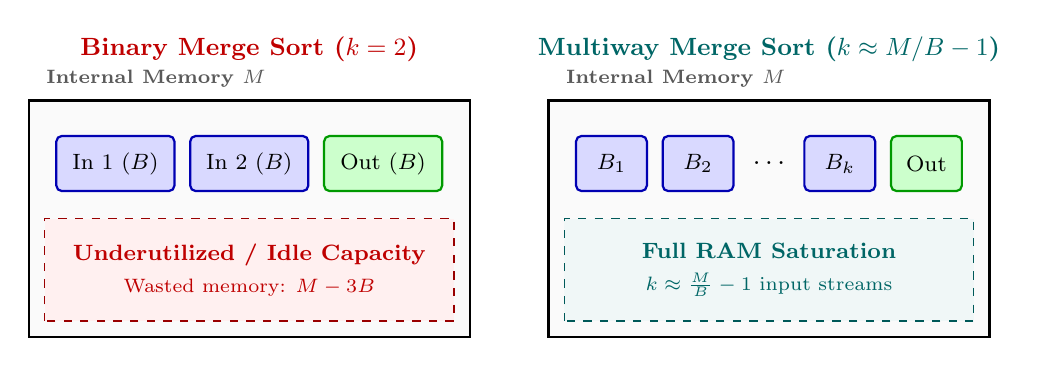
\begin{tikzpicture}[
    box/.style={draw, thick, rounded corners=2pt, align=center, font=\footnotesize},
    title/.style={font=\bfseries\small, align=center}
  ]
    % --- LEFT: Binary Merge Sort ---
    \node[title, color=red!75!black] at (2.8, 3.65) {Binary Merge Sort ($k=2$)};
    % Internal memory container M
    \draw[thick, fill=gray!4] (0, 0) rectangle (5.6, 3.0);
    \node[anchor=south west, font=\scriptsize\bfseries, color=gray!70!black] at (0.1, 3.05) {Internal Memory $M$};

    % Buffer 1, 2, Out
    \node[box, fill=blue!15, draw=blue!70!black, minimum width=1.5cm, minimum height=0.7cm] at (1.1, 2.2) {In 1 ($B$)};
    \node[box, fill=blue!15, draw=blue!70!black, minimum width=1.5cm, minimum height=0.7cm] at (2.8, 2.2) {In 2 ($B$)};
    \node[box, fill=green!20, draw=green!60!black, minimum width=1.5cm, minimum height=0.7cm] at (4.5, 2.2) {Out ($B$)};

    % Wasted space
    \draw[dashed, red!60!black, fill=red!6] (0.2, 0.2) rectangle (5.4, 1.5);
    \node[font=\footnotesize\bfseries, color=red!75!black, align=center] at (2.8, 0.85) {Underutilized / Idle Capacity\\[2pt]{\normalfont\scriptsize Wasted memory: $M - 3B$}};

    % --- RIGHT: Multiway Merge Sort ---
    \node[title, color=teal!80!black] at (9.4, 3.65) {Multiway Merge Sort ($k \approx M/B - 1$)};
    % Internal memory container M
    \draw[thick, fill=gray!4] (6.6, 0) rectangle (12.2, 3.0);
    \node[anchor=south west, font=\scriptsize\bfseries, color=gray!70!black] at (6.7, 3.05) {Internal Memory $M$};

    % Multiple buffers
    \node[box, fill=blue!15, draw=blue!70!black, minimum width=0.9cm, minimum height=0.7cm] at (7.4, 2.2) {$B_1$};
    \node[box, fill=blue!15, draw=blue!70!black, minimum width=0.9cm, minimum height=0.7cm] at (8.5, 2.2) {$B_2$};
    \node[font=\bfseries] at (9.4, 2.2) {$\dots$};
    \node[box, fill=blue!15, draw=blue!70!black, minimum width=0.9cm, minimum height=0.7cm] at (10.3, 2.2) {$B_k$};
    \node[box, fill=green!20, draw=green!60!black, minimum width=0.9cm, minimum height=0.7cm] at (11.4, 2.2) {Out};

    % Full saturation
    \draw[dashed, teal!70!black, fill=teal!6] (6.8, 0.2) rectangle (12.0, 1.5);
    \node[font=\footnotesize\bfseries, color=teal!80!black, align=center] at (9.4, 0.85) {Full RAM Saturation\\[2pt]{\normalfont\scriptsize $k \approx \frac{M}{B}-1$ input streams}};
  \end{tikzpicture}%
  }
  \caption{Internal memory allocation efficiency: severe underutilization in Binary Merge Sort versus full buffer saturation in Multiway Merge Sort.}
  \label{fig:memory-utilization-comparison}
\end{figure}

Overcoming this structural limitation leads naturally to the multiway merging architecture, which we investigate in detail in the following sections.

\section{Asymptotic Equivalence of the External Sorting Cost}
\label{sec:sorting-cost-equivalence}

In the computational analysis of secondary memory algorithms, the I/O complexity of external sorting is expressed in the literature~\cite{aggarwal1988} using two seemingly distinct formulations:
\begin{equation}
  \Theta\left(\frac{n}{B} \log_{M/B}\left(\frac{n}{M}\right)\right)
  \qquad \text{or} \qquad
  \mathcal{O}\left(\frac{n}{B} \log_{M/B}\left(\frac{n}{B}\right)\right).
\end{equation}
These two expressions are asymptotically equivalent for any problem instance where $n \ge M$.

To establish this equivalence formally, we apply the logarithmic product rule to expand the logarithmic term $\log_{M/B}(n/B)$:
\begin{align}
  \log_{M/B}\left(\frac{n}{B}\right)
  &= \log_{M/B}\left(\frac{n}{M} \cdot \frac{M}{B}\right) \nonumber \\
  &= \log_{M/B}\left(\frac{n}{M}\right) + \log_{M/B}\left(\frac{M}{B}\right) \nonumber \\
  &= \log_{M/B}\left(\frac{n}{M}\right) + 1.
  \label{eq:log-equivalence}
\end{align}
Multiplying the entire equation by the common scale factor $\frac{n}{B}$, we obtain:
\begin{equation}
  \frac{n}{B} \log_{M/B}\left(\frac{n}{B}\right)
  = \frac{n}{B} \log_{M/B}\left(\frac{n}{M}\right) + \frac{n}{B}.
\end{equation}
Algorithmically, the additional linear scan term $\frac{n}{B}$ corresponds precisely to the initial pass (Phase 0) that creates the initial sorted runs by loading chunks of size $M$ into RAM, sorting them internally, and flushing them back to disk.

Whenever $n \gg M$, we have $\log_{M/B}(n/M) \ge 1$, which implies that the additive $+1$ term is readily subsumed by the hidden constant within asymptotic $\Theta$-notation:
\begin{equation}
  \Theta\left(\frac{n}{B} \log_{M/B}\left(\frac{n}{B}\right)\right)
  = \Theta\left(\frac{n}{B} \left(\log_{M/B}\left(\frac{n}{M}\right) + 1\right)\right)
  = \Theta\left(\frac{n}{B} \log_{M/B}\left(\frac{n}{M}\right)\right).
\end{equation}
Consequently, one may freely choose either $\frac{n}{M}$ or $\frac{n}{B}$ as the argument of the logarithm without altering the asymptotic validity of the result.

\section{Multiway Merge Sort (\texorpdfstring{$k$}{k}-Way Merge Sort)}
\label{sec:multiway-merge-sort}

In the external \textit{Binary Merge Sort} presented in \autoref{sec:binary-merge-sort}, only 3 blocks of internal memory were concurrently active, wasting the remaining $M - 3B$ elements of fast storage. The \textbf{Multiway Merge Sort} (or $k$-way merge sort) overcomes this severe bottleneck by utilizing the entire capacity $M$ to merge $k$ sorted runs simultaneously in a single pass (\textit{fan-in} equal to $k$).

\subsection{Internal Memory Configuration and Layout}
\label{subsec:multiway-memory-layout}

Primary memory $M$ is partitioned into blocks of transfer size $B$:
\begin{itemize}
  \item $k = \frac{M}{B} - 1$ \textbf{input buffers}, each having capacity $B$, statically associated with one active run on external disk storage.
  \item $1$ \textbf{output buffer}, also of capacity $B$, dedicated to incrementally accumulating sorted elements before performing an I/O flush to disk.
  \item An auxiliary in-memory data structure: a \textbf{Min-Heap} (or priority queue) of cardinality $k$. Each heap node stores the current leading key of one of the $k$ active input buffers along with an identifier indicating its source buffer.
\end{itemize}

\autoref{fig:multiway-merge-architecture} illustrates the architectural buffer layout and the data flow coordinated by the Min-Heap.

\begin{figure}[H]
  \centering
  \resizebox{0.95\linewidth}{!}{%
  \begin{tikzpicture}[
    buf/.style={draw=blue!70!black, thick, fill=blue!10, rounded corners=2pt, minimum width=2.4cm, minimum height=0.75cm, align=center, font=\small},
    heap/.style={draw=orange!80!black, thick, fill=orange!15, rounded corners=4pt, minimum width=2.8cm, minimum height=1.4cm, align=center, font=\small\bfseries},
    outbuf/.style={draw=green!60!black, thick, fill=green!15, rounded corners=2pt, minimum width=2.8cm, minimum height=0.75cm, align=center, font=\small\bfseries},
    disk/.style={draw=gray!70!black, thick, fill=gray!12, rounded corners=2pt, minimum width=3.2cm, minimum height=0.8cm, align=center, font=\small},
    arr/.style={-{Stealth[scale=1.1]}, thick}
  ]
    % Internal Memory Container
    \draw[thick, dashed, fill=blue!2, draw=blue!60!black] (-0.3, -0.2) rectangle (12.2, 5.0);
    \node[anchor=south west, font=\small\bfseries, color=blue!70!black] at (-0.2, 5.05) {Internal Memory $M$ (Capacity: $k+1$ blocks)};

    % Input Buffers
    \node[buf] (b1) at (1.6, 4.1) {Input Buffer $1$ ($B$)};
    \node[buf] (b2) at (1.6, 3.1) {Input Buffer $2$ ($B$)};
    \node[font=\bfseries] at (1.6, 2.2) {$\vdots$};
    \node[buf] (bk) at (1.6, 1.2) {Input Buffer $k$ ($B$)};

    % External Disks
    \node[disk] (d1) at (-4.2, 4.1) {Active Run $1$ (Disk)};
    \node[disk] (d2) at (-4.2, 3.1) {Active Run $2$ (Disk)};
    \node[disk] (dk) at (-4.2, 1.2) {Active Run $k$ (Disk)};

    \draw[arr, color=blue!80!black] (d1) -- node[above, font=\scriptsize]{Read $B$} (b1);
    \draw[arr, color=blue!80!black] (d2) -- node[above, font=\scriptsize]{Read $B$} (b2);
    \draw[arr, color=blue!80!black] (dk) -- node[above, font=\scriptsize]{Read $B$} (bk);

    % Min-Heap in the center
    \node[heap] (hp) at (6.0, 2.6) {Min-Heap\\{\normalfont\footnotesize Size $k = \frac{M}{B}-1$}};

    % Connections from buffers to heap
    \draw[arr, color=orange!80!black] (b1.east) -- (hp.160);
    \draw[arr, color=orange!80!black] (b2.east) -- (hp.175);
    \draw[arr, color=orange!80!black] (bk.east) -- (hp.195);

    % Output Buffer
    \node[outbuf] (bout) at (10.6, 2.6) {Output Buffer ($B$)};
    \draw[arr, color=orange!80!black] (hp.east) -- node[above, font=\scriptsize\bfseries]{Minimum} (bout.west);

    % Output Disk
    \node[disk, fill=green!10, draw=green!60!black] (dout) at (10.6, -1.5) {Merged Run on Disk\\(Capacity $k \cdot l$)};
    \draw[arr, color=green!60!black] (bout.south) -- node[right, font=\scriptsize\bfseries]{Flush $B$ (1 I/O)} (dout.north);
  \end{tikzpicture}%
  }
  \caption{Internal memory layout during multiway merging ($k$-Way Merge Sort) with coordinating Min-Heap.}
  \label{fig:multiway-merge-architecture}
\end{figure}

The Min-Heap allows extracting the global minimum among all $k$ streams in $\mathcal{O}(\log_2 k)$ internal CPU comparisons. When the input buffer supplying the minimum is exhausted, a single disk read I/O is performed to load the next block of $B$ elements from that run. Similarly, each time the output buffer accumulates $B$ sorted elements, a single physical write I/O flushes the block to secondary storage.

\subsection{Algorithm Execution and Tree Height Evolution}
\label{subsec:multiway-dynamics}

The execution proceeds across two distinct phases:

\begin{enumerate}
  \item \textbf{Phase 0 (Initial Run Formation):}
  The unsorted array of $n$ elements stored on disk is streamed in chunks of size $M$. Each chunk of $M$ elements is brought into RAM, sorted using an optimal in-memory algorithm (e.g., QuickSort or HeapSort), and flushed back to disk:
  \begin{itemize}
    \item Number of initial sorted runs:
    \begin{equation}
      N_0 = \frac{n}{M}.
    \end{equation}
    \item I/O cost of Phase 0: full read and write scan across all $n$ elements:
    \begin{equation}
      \mathrm{I/O}_{\text{RunFormation}} = 2 \cdot \frac{n}{B} = \mathcal{O}\left(\frac{n}{B}\right).
    \end{equation}
  \end{itemize}

  \item \textbf{Subsequent Multiway Merging Passes ($k$-Way Merge):}
  At each level of the recursion tree, existing runs are partitioned into groups of size $k$. Each group of $k$ runs, each of current length $l$, is merged simultaneously to yield a single consolidated run of size $k \cdot l$:
  \begin{itemize}
    \item I/O cost for merging a single group of runs: $\mathcal{O}\left(\frac{k \cdot l}{B}\right)$.
    \item Total I/O cost per merge level: because every element belongs to exactly one group per level, all $n$ elements are read and written exactly once per pass, resulting in:
    \begin{equation}
      \mathrm{I/O}_{\text{Level}} = 2 \cdot \frac{n}{B} = \mathcal{O}\left(\frac{n}{B}\right).
    \end{equation}
  \end{itemize}
\end{enumerate}

At the $i$-th level of the multiway merge tree, every run has size $k^i \cdot M$. The merge process terminates when only a single consolidated run of size $n$ remains:
\begin{equation}
  k^i \cdot M = n \implies k^i = \frac{n}{M} \implies i = \log_k\left(\frac{n}{M}\right) \text{ levels}.
\end{equation}
Setting the fan-in to its maximum feasible capacity $k \approx \frac{M}{B} - 1 = \Theta\left(\frac{M}{B}\right)$, we obtain:
\begin{equation}
  \text{Number of Merge Passes} = \mathcal{O}\left(\log_{M/B}\left(\frac{n}{M}\right)\right).
\end{equation}

In \autoref{fig:multiway-merge-tree}, we illustrate the hierarchy of $k$-way merge levels, highlighting the expanded fan-in and per-level I/O scan costs throughout the recursion tree.

\begin{figure}[H]
  \centering
  \resizebox{0.95\linewidth}{!}{%
  \begin{tikzpicture}[
    run/.style={draw=blue!75!black, rounded corners=3pt, fill=blue!10, font=\small, minimum height=0.7cm, align=center},
    run0/.style={draw=orange!80!black, rounded corners=3pt, fill=orange!15, font=\footnotesize, minimum height=0.6cm, minimum width=0.65cm, align=center},
    cost/.style={font=\small, text=blue!85!black, anchor=west},
    lbl/.style={font=\small\bfseries, text=gray!80!black, anchor=east},
    arr/.style={-{Stealth[scale=0.85]}, thick, draw=gray!65!black}
  ]
    % Root Level (Top): Final run of size n
    \node[run, fill=green!15, draw=green!60!black, minimum width=3.8cm, font=\small\bfseries] (root) at (0, 0) {Final Run: $n$ elements};

    % Level 1: Intermediate runs of size k*M
    \node[run, minimum width=2.1cm] (r1_1) at (-3.4, -1.8) {Run $kM$};
    \node[run, minimum width=2.1cm] (r1_2) at (-1.0, -1.8) {Run $kM$};
    \node[font=\bfseries] at (0.7, -1.8) {$\dots$};
    \node[run, minimum width=2.1cm] (r1_k) at (2.4, -1.8) {Run $kM$};

    % Arrows from Level 1 to root (k-way merge)
    \draw[arr] (r1_1.north) -- (root.south west);
    \draw[arr] (r1_2.north) -- (root.south);
    \draw[arr] (r1_k.north) -- (root.south east);

    % Level 0: Group 1 (centered below r1_1 at x=-3.4)
    \node[run0] (r0_1) at (-4.1, -3.7) {$M$};
    \node[font=\scriptsize] at (-3.4, -3.7) {$\dots$};
    \node[run0] (r0_k) at (-2.7, -3.7) {$M$};

    \draw[arr] (r0_1.north) -- (r1_1.south west);
    \draw[arr] (r0_k.north) -- (r1_1.south east);

    % Group 2 (centered below r1_2 at x=-1.0)
    \node[run0] (r0_k1) at (-1.7, -3.7) {$M$};
    \node[font=\scriptsize] at (-1.0, -3.7) {$\dots$};
    \node[run0] (r0_2k) at (-0.3, -3.7) {$M$};

    \draw[arr] (r0_k1.north) -- (r1_2.south west);
    \draw[arr] (r0_2k.north) -- (r1_2.south east);

    % Final group k (centered below r1_k at x=2.4)
    \node[font=\scriptsize] at (0.7, -3.7) {$\dots$};
    \node[run0] (r0_end1) at (1.7, -3.7) {$M$};
    \node[font=\scriptsize] at (2.4, -3.7) {$\dots$};
    \node[run0] (r0_end2) at (3.1, -3.7) {$M$};

    \draw[arr] (r0_end1.north) -- (r1_k.south west);
    \draw[arr] (r0_end2.north) -- (r1_k.south east);

    % Braces for base groups
    \draw[thick, decorate, decoration={brace, mirror, amplitude=4pt}] (-4.25, -4.15) -- (-2.55, -4.15)
      node[midway, below=5pt, font=\scriptsize] {$k$ runs};
    \draw[thick, decorate, decoration={brace, mirror, amplitude=4pt}] (-1.85, -4.15) -- (-0.15, -4.15)
      node[midway, below=5pt, font=\scriptsize] {$k$ runs};
    \draw[thick, decorate, decoration={brace, mirror, amplitude=4pt}] (1.55, -4.15) -- (3.25, -4.15)
      node[midway, below=5pt, font=\scriptsize] {$k$ runs};

    % Left labels with explicit k-way merge indicators
    \node[lbl] at (-5.0, 0) {Level $h = \log_k\left(\frac{n}{M}\right)$:};
    \node[font=\scriptsize\bfseries, color=blue!85!black, anchor=east] at (-5.0, -0.9) {$\uparrow$ $k$-way merge ($k \approx M/B$)};
    \node[lbl] at (-5.0, -1.8) {Level $1$:};
    \node[font=\scriptsize\bfseries, color=blue!85!black, anchor=east] at (-5.0, -2.75) {$\uparrow$ $k$-way merge ($k \approx M/B$)};
    \node[lbl] at (-5.0, -3.7) {Level $0$ (Base):};

    % Right dashed lines to I/O costs
    \draw[dotted, thick, gray!45] (root.east) -- (4.0, 0);
    \node[cost] at (4.1, 0) {$2\frac{n}{B}$ I/O};

    \draw[dotted, thick, gray!45] (r1_k.east) -- (4.0, -1.8);
    \node[cost] at (4.1, -1.8) {$2\frac{n}{B}$ I/O};

    \draw[dotted, thick, gray!45] (r0_end2.east) -- (4.0, -3.7);
    \node[cost] at (4.1, -3.7) {$2\frac{n}{B}$ I/O (Phase 0)};

    % Tree height arrow positioned at x=7.6 well clear of "(Phase 0)"
    \draw[thick, Stealth-Stealth, color=red!70!black] (7.6, 0.2) -- 
      node[right=4pt, font=\small, text=red!80!black, align=left]{$h = \log_k\left(\frac{n}{M}\right)$\\[2pt]passes} 
      (7.6, -3.9);
  \end{tikzpicture}%
  }
  \caption{Level evolution and $k$-way merge tree in Multiway Merge Sort.}
  \label{fig:multiway-merge-tree}
\end{figure}

Combining both phases gives the overall I/O complexity:
\begin{equation}
  \begin{aligned}
    \mathrm{I/O}_{\text{Total}}
    &= \underbrace{\mathcal{O}\left(\frac{n}{B}\right)}_{\text{Run Formation}} + \underbrace{\mathcal{O}\left(\frac{n}{B} \log_{M/B}\left(\frac{n}{M}\right)\right)}_{\text{Merging Passes}} \\
    &= \mathcal{O}\left(\frac{n}{B} \log_{M/B}\left(\frac{n}{B}\right)\right) \text{ I/O operations}.
  \end{aligned}
\end{equation}
This matches the asymptotic lower bound for hierarchical memory sorting established by Aggarwal and Vitter~\cite{aggarwal1988}, proving that Multiway Merge Sort is asymptotically optimal.

\section{Optimizing Run Formation: The Snow Plow (\texorpdfstring{\emph{Replacement Selection}}{Replacement Selection})}
\label{sec:snow-plow}

While standard Multiway Merge Sort creates initial runs of length bounded by memory capacity $M$, the tree depth $\lceil \log_{M/B}(n/M) \rceil$ depends directly on the initial number of runs. Producing runs substantially longer than $M$ flattens the merge tree and can eliminate an entire I/O pass across petabyte-scale datasets.

A foundational technique designed to achieve this is \textbf{Replacement Selection}, historically known by the vivid metaphor of the \textbf{Snow Plow}~\cite{knuth1997}.

\subsection{Operational Mechanism of Replacement Selection}
\label{subsec:snow-plow-mechanism}

Rather than statically filling memory $M$, sorting it, and flushing it in bulk, the algorithm keeps fast memory $M$ fully occupied at all times by dynamically splitting it into two logical partitions:
\begin{itemize}
  \item \textbf{Active Elements (Current Min-Heap):} elements whose keys are greater than or equal to the last element emitted to the current run on disk. These elements are valid candidates to append to the active run.
  \item \textbf{Frozen Elements ($U$):} newly ingested elements whose keys are strictly smaller than the last element emitted. Appending them would violate the sorted invariant; hence they are ``frozen'' in RAM, waiting for the subsequent run.
\end{itemize}

\autoref{fig:snow-plow-partition} shows the dynamic memory partitioning during the snow plow sweep.

\begin{figure}[H]
  \centering
  \resizebox{0.95\linewidth}{!}{%
  \begin{tikzpicture}[
    box/.style={draw=blue!75!black, thick, fill=blue!10, rounded corners=3pt, minimum height=1.7cm, align=center, text width=5.9cm, font=\small},
    frozen/.style={draw=teal!75!black, thick, fill=teal!12, rounded corners=3pt, minimum height=1.7cm, align=center, text width=5.8cm, font=\small}
  ]
    % Total memory M container with generous padding
    \draw[thick, draw=gray!70!black, fill=gray!5, rounded corners=4pt] (0, -0.65) rectangle (14.2, 3.4);
    \node[anchor=south west, font=\small\bfseries, color=gray!80!black] at (0.1, 3.45) {Primary Memory $M$ (Total Shared Capacity Dynamically Partitioned)};

    % Block 1: Active Elements
    \node[box] (active) at (3.5, 1.7) {%
      \textbf{Active Partition (Min-Heap)}\\[3pt]%
      \footnotesize Keys $\ge \text{last\_emitted}$\\[2pt]%
      \scriptsize (Eligible for current run)%
    };

    % Block 2: Frozen Elements
    \node[frozen] (froz) at (10.7, 1.7) {%
      \textbf{Frozen Partition (Set $U$)}\\[3pt]%
      \footnotesize Keys $< \text{last\_emitted}$\\[2pt]%
      \scriptsize (Parked for next run)%
    };

    % Dynamic boundary between both blocks
    \draw[very thick, dashed, draw=red!75!black] (7.1, 0.45) -- (7.1, 2.85);
    \node[font=\scriptsize\bfseries, fill=white, inner sep=2pt, text=red!75!black, rounded corners=2pt, draw=red!40] at (7.1, 2.95) {Dynamic Boundary};

    % Bottom arrow showing snow plow progression
    \draw[-{Stealth[scale=1.0]}, thick, draw=red!75!black] (5.8, -0.1) -- (8.4, -0.1);
    \node[font=\scriptsize\bfseries, text=red!75!black, anchor=north] at (7.1, -0.18) {Growth of $U$ (until $\vert U\vert = M$)};
  \end{tikzpicture}%
  }
  \caption{Dynamic partitioning of memory $M$ during Replacement Selection (Snow Plow).}
  \label{fig:snow-plow-partition}
\end{figure}

The algorithm executes the following element-wise loop:
\begin{enumerate}
  \item Extract the minimum active element from the root of the Min-Heap, write it to the output buffer, and record its key as $\text{last\_emitted}$.
  \item Ingest the next item $x$ from the unsorted input stream:
  \begin{itemize}
    \item If $x \ge \text{last\_emitted}$, insert $x$ into the active Min-Heap.
    \item If $x < \text{last\_emitted}$, assign $x$ to the frozen set $U$.
  \end{itemize}
  \item The active run terminates when the active heap becomes empty, i.e., when all $M$ memory slots are occupied by frozen elements ($\vert{}U\vert{} = M$). At this moment, set $U$ is transformed into the new active Min-Heap, a new run file is opened on disk, and the cycle repeats.
\end{enumerate}

\subsection{Step-by-Step Execution Trace}
\label{subsec:snow-plow-trace}

Consider internal memory capacity $M = 3$ and an input stream:
\[
  S = [1, \, 7, \, 5, \, 3, \, 2, \, 9, \, 0, \, 4, \, \dots].
\]
\autoref{tab:snow-plow-trace} traces the step-by-step state of memory and the output stream.

\begin{table}[H]
  \centering
  \caption{Execution trace of Replacement Selection with capacity $M=3$.}
  \label{tab:snow-plow-trace}
  \small
  \setlength{\tabcolsep}{4pt}
  \begin{tabularx}{\textwidth}{c c c Y c c}
    \toprule
    \textbf{Step} & \textbf{Active} & \textbf{Frozen ($U$)} & \textbf{Action Performed} & \textbf{Emitted} & \textbf{Run} \\
    \midrule
    \textbf{0} & $\{1, 5, 7\}$ & $\emptyset$ & Initial load of $M=3$ items & — & $[\,]$ \\
    \textbf{1} & $\{5, 7\}$ & $\emptyset$ & Emit $1$; read $3$. Since $3 \ge 1$, remains active & \textbf{1} & $[1]$ \\
    \textbf{2} & $\{5, 7\}$ & $\emptyset$ & Emit $3$; read $2$. Since $2 < 3$, \textbf{$2$ goes to $U$} & \textbf{3} & $[1, 3]$ \\
    \textbf{3} & $\{7, 9\}$ & $\{2\}$ & Emit $5$; read $9$. Since $9 \ge 5$, remains active & \textbf{5} & $[1, 3, 5]$ \\
    \textbf{4} & $\{9\}$ & $\{2, 0\}$ & Emit $7$; read $0$. Since $0 < 7$, \textbf{$0$ goes to $U$} & \textbf{7} & $[1, 3, 5, 7]$ \\
    \textbf{5} & $\emptyset$ & $\{2, 0, 4\}$ & Emit $9$; read $4$. Since $4 < 9$, \textbf{$4$ goes to $U$} & \textbf{9} & $[1, 3, 5, 7, 9]$ \\
    \bottomrule
  \end{tabularx}
\end{table}

At Step 5, active memory is completely depleted and frozen items fill all $M$ slots: $\vert{}U\vert{} = M = 3$. The current run closes with a length of \textbf{5 items}—significantly exceeding physical memory capacity $M = 3$. The frozen set $\{0, 2, 4\}$ immediately forms the seed heap for the subsequent run.

\paragraph{Note on Production Systems.}
In production databases and file systems, transfers are performed using blocks of size $B$ rather than single elements, utilizing prefetching buffers and write accumulation buffers (\textit{double buffering}) without altering the asymptotic I/O behavior.

\subsection{Average Run Length Theorem}
\label{subsec:snow-plow-theorem}

\begin{theorem}[Average Run Length in Snow Plow]
\label{thm:snow-plow-length}
Assuming that input keys are independent and identically distributed random variables drawn from a continuous uniform distribution, the average run length produced by Replacement Selection is asymptotically $2M$.
\end{theorem}

\begin{proof}[Heuristic Proof]
We analyze the steady-state stochastic process:
\begin{enumerate}
  \item At the start of a run, memory holds $M$ elements.
  \item Let $\tau$ denote the number of additional items read from the input before the run ends. The total run length is $M + \tau$.
  \item The run concludes when the frozen buffer reaches full capacity: $\vert{}U\vert{} = M$.
  \item By distributional symmetry and statistical independence, each incoming element has probability $P = \frac{1}{2}$ of being smaller than the last emitted element (landing in $U$) and probability $P = \frac{1}{2}$ of being greater than or equal to it (joining the active run).
  \item The expected number of items placed in $U$ after reading $\tau$ elements is:
  \begin{equation}
    \mathbb{E}[\vert{}U\vert{}] = \tau \cdot P(\text{placed into } U) = \tau \cdot \frac{1}{2}.
  \end{equation}
  \item Equating this expectation to the termination threshold $\mathbb{E}[\vert{}U\vert{}] = M$:
  \begin{equation}
    \frac{\tau}{2} = M \implies \tau = 2M.
  \end{equation}
\end{enumerate}
Consequently, the expected average run length is approximately $2M$.
\end{proof}

Doubling the average run length ($\approx 2M$) cuts the initial number of runs in half $\left(\frac{n}{2M}\right)$, directly decreasing the required number of full I/O passes across the dataset.

\section{Parallelism Across Multiple Disks: \texorpdfstring{\emph{Disk Striping}}{Disk Striping}}
\label{sec:disk-striping}

In modern data centers and high-performance computing clusters, secondary storage is distributed across $D$ independent physical disk drives or SSD units.

\subsection{Parallel External Sorting Lower Bound}
\label{subsec:parallel-lower-bound}

When a storage architecture incorporates $D$ parallel disk units, each capable of transferring one block $B$ per I/O cycle, the Aggarwal-Vitter~\cite{aggarwal1988} lower bound scales with an ideal factor $D$ in the denominator:
\begin{equation}
  \operatorname{Sort}_D(n, M, B) = \Omega\left(\frac{n}{D \cdot B} \log_{M/B}\left(\frac{n}{M}\right)\right) \text{ parallel I/O steps}.
\end{equation}

However, designing an algorithm that achieves this lower bound using asynchronous independent disks is remarkably intricate: one must continuously prevent disk contention and bottlenecking where access concentrates on a single drive while $D-1$ drives sit idle.

\subsection{The Disk Striping Technique}
\label{subsec:striping-architecture}

To exploit physical parallelism without introducing complex asynchronous disk schedulers, systems employ \textbf{Disk Striping} (analogous to RAID 0 architecture):
\begin{itemize}
  \item The $D$ physical disks $d_1, d_2, \dots, d_D$ are logically aggregated into a single unified volume.
  \item A \textbf{logical super-block} of aggregate size:
  \begin{equation}
    B' = D \cdot B
  \end{equation}
  is defined by combining one physical block of size $B$ stored at the identical track or cylinder position on each of the $D$ drives.
  \item Every I/O transfer operates on an entire super-block of size $B'$, distributing the I/O load synchronously and uniformly across all $D$ channels in a single parallel transfer cycle.
\end{itemize}

\autoref{fig:disk-striping-architecture} illustrates the mapping of super-block $B'$ onto the $D$ underlying physical disks.

\begin{figure}[H]
  \centering
  \begin{tikzpicture}[
    dsk/.style={draw=blue!70!black, thick, fill=blue!10, rounded corners=2pt, minimum width=2.2cm, minimum height=0.75cm, align=center, font=\small},
    sblk/.style={draw=green!60!black, thick, fill=green!15, rounded corners=4pt, minimum width=3.8cm, minimum height=1.1cm, align=center, font=\small\bfseries},
    arr/.style={-{Stealth[scale=1.1]}, thick}
  ]
    \node[dsk] (d1) at (0, 2.5) {Disk $1$\\Block $B$};
    \node[dsk] (d2) at (0, 1.3) {Disk $2$\\Block $B$};
    \node[font=\bfseries] at (0, 0.4) {$\vdots$};
    \node[dsk] (dD) at (0, -0.6) {Disk $D$\\Block $B$};

    \node[sblk] (sb) at (6.5, 0.95) {Logical Super-Block\\$B' = D \cdot B$\\{\normalfont\scriptsize Transferred in $1$ Parallel I/O}};

    \draw[arr, color=blue!70!black] (d1.east) -- (sb.160);
    \draw[arr, color=blue!70!black] (d2.east) -- (sb.175);
    \draw[arr, color=blue!70!black] (dD.east) -- (sb.200);
  \end{tikzpicture}
  \caption{Disk striping layout: aggregating $D$ physical blocks into a single logical super-block $B'$.}
  \label{fig:disk-striping-architecture}
\end{figure}

Executing Multiway Merge Sort using logical block size $B'$, the number of super-blocks is $\frac{n}{B'} = \frac{n}{D \cdot B}$, while the memory fan-in capacity becomes $\frac{M}{B'} = \frac{M}{D \cdot B}$. The parallel I/O complexity is:
\begin{equation}
  \mathrm{I/O}_{\text{Striping}} = \mathcal{O}\left(\frac{n}{B'} \log_{M/B'}\left(\frac{n}{M}\right)\right) = \mathcal{O}\left(\frac{n}{D \cdot B} \log_{\frac{M}{D \cdot B}}\left(\frac{n}{M}\right)\right).
\end{equation}

\subsection{Slowdown Analysis}
\label{subsec:striping-slowdown}

Although Disk Striping achieves full bandwidth utilization across all $D$ channels, it reduces the available merging fan-in from $\frac{M}{B}$ down to $\frac{M}{D \cdot B}$, because each open run requires a buffer of size $B' = D \cdot B$.

To quantify this loss of efficiency relative to the optimal independent-disk lower bound, we compute the ratio of their I/O complexities (\textit{Slowdown}):
\begin{equation}
  \text{Slowdown} = \frac{\mathrm{I/O}_{\text{Striping}}}{\mathrm{I/O}_{\text{Ideal}}}
  = \frac{\displaystyle \frac{n}{D \cdot B} \log_{\frac{M}{D \cdot B}}\left(\frac{n}{M}\right)}{\displaystyle \frac{n}{D \cdot B} \log_{\frac{M}{B}}\left(\frac{n}{M}\right)}
  = \frac{\log_{\frac{M}{D \cdot B}}\left(\frac{n}{M}\right)}{\log_{\frac{M}{B}}\left(\frac{n}{M}\right)}.
\end{equation}
Changing the logarithm base to $2$ using $\log_a x = \frac{\log_2 x}{\log_2 a}$:
\begin{equation}
  \text{Slowdown} = \frac{\displaystyle \frac{\log_2(n / M)}{\log_2(M / (D \cdot B))}}{\displaystyle \frac{\log_2(n / M)}{\log_2(M / B)}}
  = \frac{\log_2(M / B)}{\log_2(M / (D \cdot B))}
  = \frac{\log_2(M / B)}{\log_2(M / B) - \log_2 D}.
\end{equation}
Dividing numerator and denominator by $\log_2(M / B)$:
\begin{equation}
  \text{Slowdown} = \frac{1}{\displaystyle 1 - \frac{\log_2 D}{\log_2(M / B)}}.
  \label{eq:slowdown-formula}
\end{equation}

\subsection{Asymptotic Regimes and Physical Limitations}
\label{subsec:striping-limits}

The behavior of the slowdown factor is governed entirely by the dimensionless ratio:
\begin{equation}
  \rho = \frac{\log_2 D}{\log_2(M / B)}.
\end{equation}
Two limiting operating regimes arise:

\begin{enumerate}
  \item \textbf{Ample Memory Regime ($M \to \infty$ or $D \ll \frac{M}{B}$):}
  When RAM is substantially larger than the number of attached disk drives, the memory fan-in factor dominates:
  \begin{equation}
    \rho = \frac{\log_2 D}{\log_2(M / B)} \to 0 \implies \text{Slowdown} \to \frac{1}{1 - 0} = 1.
  \end{equation}
  In this regime, Disk Striping suffers virtually no degradation and attains the asymptotic performance of the theoretical independent-disk system, representing an optimal engineering tradeoff due to its implementation simplicity.

  \item \textbf{Memory Saturation Regime ($\log_2 D \to \log_2(M/B)$):}
  When the drive count $D$ approaches the maximum number of blocks that fit into internal memory ($D \approx \frac{M}{B}$), the ratio $\rho$ approaches $1$. The denominator of \eqref{eq:slowdown-formula} tends to zero, causing the expression to diverge:
  \begin{equation}
    \lim_{\rho \to 1^-} \frac{1}{1 - \rho} = +\infty.
  \end{equation}
  \textbf{Physical interpretation:} If $D \ge \frac{M}{B}$, internal memory cannot accommodate even a single super-block $B' = D \cdot B$ per active input stream, rendering striping physically impossible and causing the multiway merge to collapse.
\end{enumerate}

